\documentclass{beamer}
\usepackage{risk201}

\setchapter{8}

% Chapter-specific diagram shortcuts
\newcommand{\fwdline}{\timeline[3,6]{8}{0/0, 1/1, 2/2, 4/t, 5/t+1, 7.5/t+m}}


\title{RISK 201: Yield Curves}

\begin{document}
\maketitle

%======================================================================
\section{Term structure of interest rates}
%======================================================================

\begin{frame}{8.1 Term structure of interest rates}

\begin{itemize}
\item The observed yields on zero-coupon bonds of different maturities is referred to collectively as the \purple{\textbf{yield curve}}. It is also known as the \purple{\textbf{term structure of interest rates}}.
\bigskip
\item The yield curve is usually increasing, meaning that zero-coupon bonds of longer maturities command a higher yield than zero-coupon bonds of shorter maturities.
\bigskip
\item Occasionally, the yield curve could be flat or decreasing (inverted).
\end{itemize}

\end{frame}

\begin{frame}{Why is the yield curve upward sloping?}

\begin{itemize}
\item Expectations Theory
\begin{itemize}
\item[] Investors expect interest rates to rise in the future
\end{itemize}
\medskip
\item Liquidity Preference Theory
\begin{itemize}
\item[] Investors need an incentive (higher yield) to tie up their money in the long term (as opposed to staying in more liquid, shorter-term investments)
\end{itemize}
\medskip
\item Inflation Risk Premium Theory
\begin{itemize}
\item[] The fixed income provided by bonds is eroded by inflation. Since future inflation is uncertain and may rise, investors need incentive to invest over longer term.
\end{itemize}
\end{itemize}

\end{frame}

\begin{frame}{Changes in the yield curve}

\begin{itemize}
\item Parallel shifts:
\begin{itemize}
\item All yields change by the same amount (e.g., 1\% up)
\end{itemize}
\medskip
\item Non-parallel shifts (twists):
\begin{itemize}
\item Different parts of the yield curve (short, medium and long maturities) shift by different amounts $\rightarrow$ slope and curvature changes
\end{itemize}
\medskip
\item Inversion:
\begin{itemize}
\item Short-term yields exceed long-term yields. Relatively rare; usually taken as a signal of an impending recession or other weakness.
\end{itemize}
\end{itemize}

\end{frame}

\begin{frame}{Observed US Treasury yields (Jan 31)}

\begin{center}
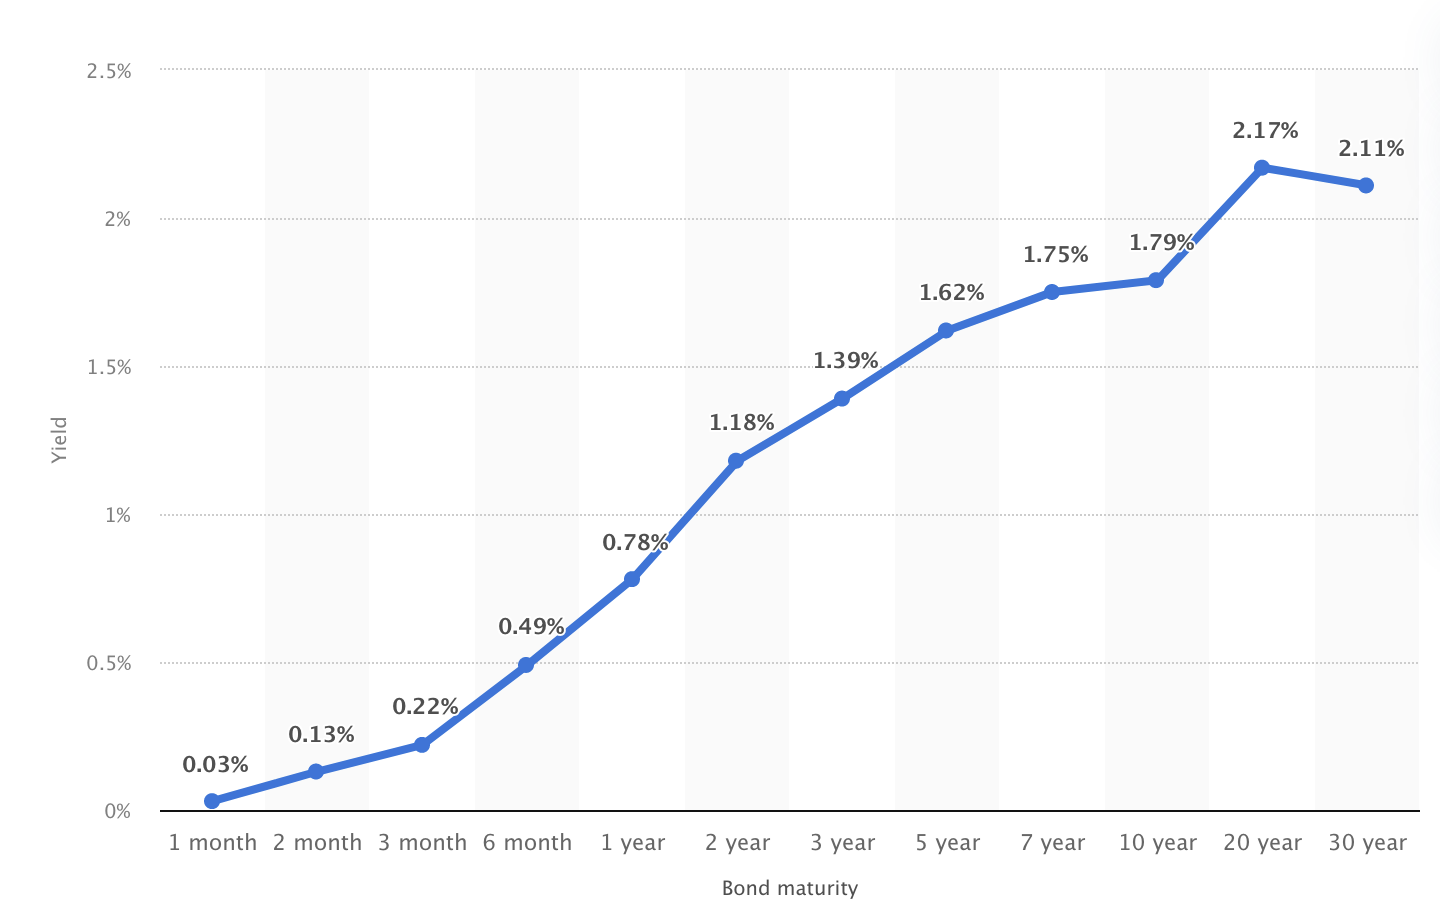
\includegraphics[width=0.95\textwidth]{figures/ch8_us_treasury_yields.png}
\end{center}

\end{frame}

\begin{frame}

\begin{center}
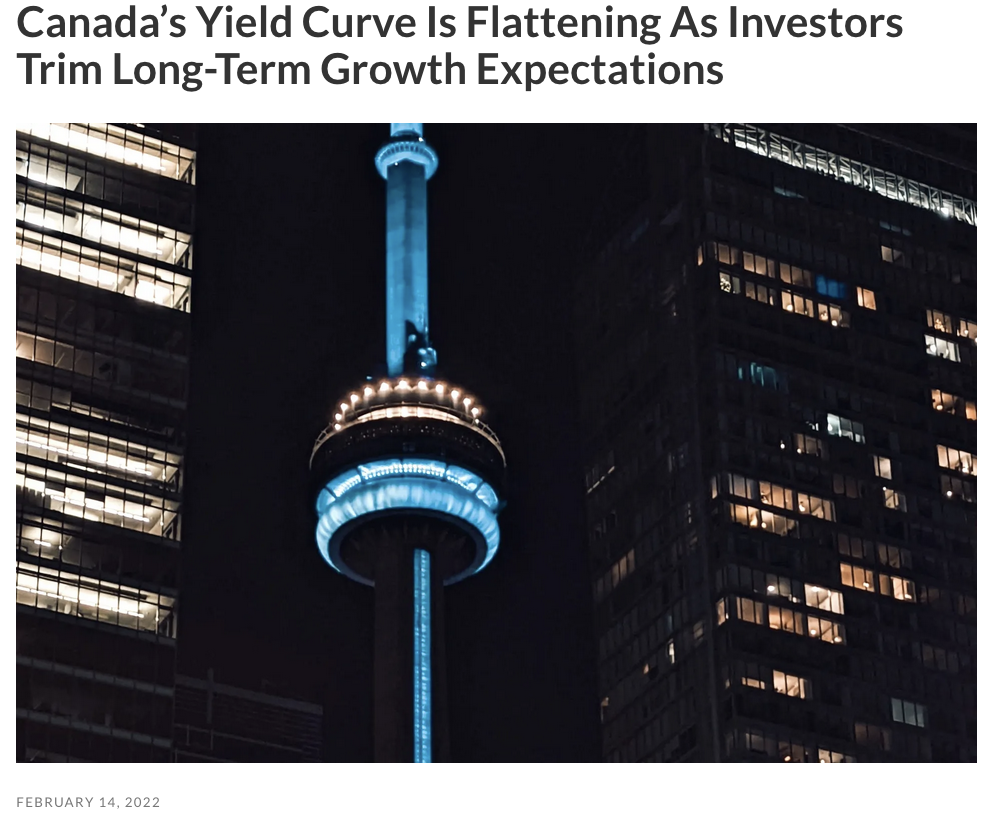
\includegraphics[height=0.88\textheight]{figures/ch8_canada_yield_curve_article.png}
\end{center}

\end{frame}

\begin{frame}{Riding the yield curve}

Consider the following strategy:
\begin{itemize}
\item Invest in a longer term (e.g., 10 year) bond
\item Instead of holding the bond to maturity, sell it before maturity (e.g., after 3 years).
\item If the yield curve is upward sloping and hasn't shifted, the YTM of the remaining bond (now with 7 years to maturity) is lower than the YTM of the original bond purchased.
\item Investor will get a higher price $\rightarrow$ enhanced yield
\end{itemize}

\end{frame}

\begin{frame}{Example 8.1}

Using the data for US Treasuries as of Jan 31:
\begin{enumerate}[(a)]
\item Determine the purchase price of a 10-year zero-coupon bond with \$1000 face value.
\vspace{6em}
\item Determine the sale price of the same zero-coupon bond 3 years later (now 7 years to maturity) assuming the yield curve has not changed.
\end{enumerate}

\vfill
\end{frame}

\begin{frame}{Example 8.1, continued}

\begin{enumerate}[(a)]
\setcounter{enumi}{2}
\item Determine the overall yield to the investor.
\end{enumerate}

\vfill
\end{frame}

%======================================================================
\section{Spot rates}
%======================================================================

\begin{frame}{8.2 Spot rates}

\begin{itemize}
\item Let \green{$S_t$} be the (annual) yield at time 0 on a zero-coupon bond with a term of $t$ years. This is called the \green{\textbf{$t$-year spot rate}}.
\medskip
\item Then, the price of a $t$-year zero coupon bond with face amount of \$1 is
\vspace{5em}
\item The zero-coupon bond yield curve, also called the spot rate curve, consists of the set of spot rates for all maturities available at a given time:
\end{itemize}

\vfill
\end{frame}

\begin{frame}{Pricing cash flows with spot rates}

Spot rates provide a way of finding the PV of cash flows that is consistent with the market value of fixed income investments:
\[
PV = \sum_{t=0}^{n} \frac{C_t}{(1+S_t)^t}
\]

\end{frame}

\begin{frame}{Example 8.2}

Suppose spot rates are: $S_1 = 1\%$, $S_2 = 2\%$.

\begin{enumerate}[(a)]
\item What would be the purchase price of a 2-year bond with face amount \$100 and annual coupons at 4\% consistent with these spot rates?
\end{enumerate}

\begin{center}
\timeline{5}{0/0, 2.5/1, 5/2}
\end{center}

\vfill
\end{frame}

\begin{frame}{Example 8.2, continued}

\begin{enumerate}[(a)]
\setcounter{enumi}{1}
\item What is the corresponding YTM?
\end{enumerate}

\vfill
\end{frame}

\begin{frame}{Replicating portfolio}

We have essentially built a \purple{\textbf{replicating portfolio}} whose cash flows exactly match the cash flows of the asset we are trying to price.

\bigskip
The \orange{\textbf{Law of One Price}} states that, in an efficient market, all securities with the same cash flows must have the same price. Imbalances and inefficiencies can only exist for a short time.

\end{frame}

\begin{frame}{Example 8.2, continued}

What would happen if we could buy the 2-year bond for \$102 instead?

\medskip
\green{Buy the 2-year bond for \$102} today and, at the same time, \purple{sell \$3.96 of one-year zeros} and \textcolor{red}{\$98.04 of two-year zeros}.

\begin{center}
\cfrows{6}{0/0, 3/1, 6/2}{dgreen/2-year bond:, purple/1-year zero:, red/2-year zero:}
\end{center}

\vfill
\end{frame}

\begin{frame}{Arbitrage}

\blue{\textbf{Arbitrage}} refers to the simultaneous purchase and sale of securities which generate a \blue{\textbf{sure}} profit from \blue{\textbf{zero}} net investment.

\bigskip
Our assumptions in Example 8.2:
\begin{itemize}
\item no transaction costs on buying and selling
\item anyone can buy/sell bonds at rates in the yield curve
\item anyone can buy/sell zero-coupon bonds at prices indicated by the spot rates
\end{itemize}

\end{frame}

\begin{frame}{Constructing the spot rate curve}

Two methods:
\begin{enumerate}
\item From actual observed yield on zero coupon bonds
\item From actual observed prices on coupon bonds
\begin{itemize}
\item Consider bonds in order of increasing maturity
\item On the one hand, price is PV of all cash flows discounted at YTM
\item Price is also the PV of each cash flow discounted at the corresponding spot rate.
\end{itemize}
\end{enumerate}

\end{frame}

\begin{frame}{Bond pricing with Spot rates/YTM}

In other words, the price of a bond can be expressed either in terms of the YTM or in terms of spot rates:
\begin{align*}
P^{YTM} &= Fr\left[\frac{1}{1+i} + \frac{1}{(1+i)^2} + \cdots + \frac{1}{(1+i)^n}\right] + \frac{C}{(1+i)^n} \\[1ex]
P^{S} &= Fr\left[\frac{1}{1+s_1} + \frac{1}{(1+s_2)^2} + \cdots + \frac{1}{(1+s_n)^n}\right] + \frac{C}{(1+s_n)^n}
\end{align*}

\end{frame}

\begin{frame}{Example 8.3}

Find the 1-, 2-, and 3-year spot rates from the following information regarding coupon bonds redeemable at par:

\begin{center}
\begin{tabular}{ccc}
\toprule
\textbf{Term} & \textbf{Annual coupon rate} & \textbf{Annual yield rate} \\
\midrule
1 & 2.000\% & 5.000\% \\
2 & 5.000\% & 5.487\% \\
3 & 5.961\% & 5.961\% \\
\bottomrule
\end{tabular}
\end{center}

\vfill
\end{frame}

\begin{frame}{Example 8.3, continued}

Price of 1-year bond:

\vspace{10em}
Price of 2-year bond:

\vfill
\end{frame}

\begin{frame}{Example 8.3, continued}

Price of 3-year bond:

\vfill
\end{frame}

\begin{frame}{Spot rates vs.\ YTM}

Recall that the price of a bond can be expressed either in terms of the YTM or in terms of spot rates:
\begin{align*}
P^{YTM} &= Fr\left[\frac{1}{1+i} + \frac{1}{(1+i)^2} + \cdots + \frac{1}{(1+i)^n}\right] + \frac{C}{(1+i)^n} \\[1ex]
P^{S} &= Fr\left[\frac{1}{1+s_1} + \frac{1}{(1+s_2)^2} + \cdots + \frac{1}{(1+s_n)^n}\right] + \frac{C}{(1+s_n)^n}
\end{align*}

\end{frame}

\begin{frame}{Spot rates vs.\ YTM}

\begin{itemize}
\item For a zero-coupon bond ($r = 0$):
\[
i =
\]
\item For a coupon bond ($r > 0$), when the yield curve is flat ($s_1 = s_2 = \cdots = s_n$):
\[
i =
\]
\item For a coupon bond, when the yield curve is increasing ($s_1 < s_2 < \cdots < s_n$):
\end{itemize}

\vfill
\end{frame}

%======================================================================
\section{Forward rates}
%======================================================================

\begin{frame}{8.3 Forward rates}

\begin{itemize}
\item A \purple{\textbf{forward rate}} is a rate of interest that can be locked in today and that applies from one specified time to another specified time in the future.
\medskip
\item For example, the \green{\textbf{one-year forward rate of interest}}, denoted by $f_1$, is the rate of interest specified \underline{now} for an investment beginning at time 1 and lasting until time 2.
\end{itemize}

\vspace{2em}
\begin{center}
\fwdline
\end{center}

\end{frame}

\begin{frame}{Forward rates}

\begin{itemize}
\item The \blue{$t$-year forward, one-year rate of interest} (aka the \blue{$t$-year forward rate}) is denoted by $f_t$. It is the rate of interest specified \underline{now} for an investment beginning at time $t$ and lasting until time $t+1$.

\begin{center}
\fwdline
\end{center}

\item The \textcolor{red}{$t$-year forward, $m$-year rate of interest}, ${}_{m}f_{t}$, is the annual rate specified \underline{now} for an investment beginning at time $t$ and lasting until time $t+m$.
\end{itemize}

\end{frame}

\begin{frame}{Spots and forwards}

Suppose we have a set of spot rates $\{s_i\}_{i=1}^{\infty}$.

\medskip
What is the 1-year forward rate in terms of spot rates?

\begin{center}
\fwdline
\end{center}

\vfill
\end{frame}

\begin{frame}{Spots and forwards, continued}

What is the $t$-year forward rate in terms of spot rates?

\begin{center}
\fwdline
\end{center}

\vfill
\end{frame}

\begin{frame}{Spots and forwards, continued}

What is the $t$-year forward, $m$-year rate, in terms of spot rates?

\begin{center}
\fwdline
\end{center}

\vspace{4em}
The following holds for the spots and forwards rates:
\[
\prod_{j=1}^{t} (1 + f_{j-1}) = (1 + s_t)^t
\]

\vfill
\end{frame}

\begin{frame}{Pricing with forward rates}

Forward rates can be used to find the present value of a series of cash flows:

\begin{center}
\timeline[3,6]{8}{0/0, 1/1, 2/2, 4/t-1, 5/t, 7.5/n}
\end{center}

\vspace{2em}
\[
PV = \sum_{t=1}^{n} \frac{C_t}{\prod_{j=1}^{t} (1 + f_{j-1})}
\]

\end{frame}

\begin{frame}{Example 8.4}

The 1-year spot rate is 4.8\%. The 1-year forward rate is 5.1\%. The 2-year forward rate is 5.3\%. Calculate the price of 3-year bond with face amount 100 redeemable at par paying 8\% annual coupons.

\vfill
\end{frame}

\begin{frame}{Extracting forward rates from YTM}

Forward rates can be extracted from the YTM on coupon bonds:
\begin{itemize}
\item Consider bonds in order of increasing maturity
\item On the one hand, price is PV of all cash flows discounted at YTM
\item Price is also the PV of each cash flow discounted using the appropriate forward rates
\end{itemize}

\end{frame}

\begin{frame}{Example 8.5}

Find the 0-, 1-, and 2-year forward rates from the following information regarding coupon bonds redeemable at par:

\begin{center}
\begin{tabular}{ccc}
\toprule
\textbf{Term} & \textbf{Annual coupon rate} & \textbf{Annual yield rate} \\
\midrule
1 & 2.000\% & 5.000\% \\
2 & 5.000\% & 5.487\% \\
3 & 5.961\% & 5.961\% \\
\bottomrule
\end{tabular}
\end{center}

\vfill
\end{frame}

\begin{frame}{Example 8.5, continued}

Price of 1-year bond:

\vspace{10em}
Price of 2-year bond:

\vfill
\end{frame}

\begin{frame}{Example 8.5, continued}

Price of 3-year bond:

\vfill
\end{frame}

\begin{frame}{Patterns of forward rates}

When the spot rate curve is flat, so are the forward rates.

\begin{center}
\timeline[3]{7}{0/0, 1/1, 2/2, 4.5/t, 6/t+1}
\end{center}

\vfill
\end{frame}

\begin{frame}{Patterns of forward rates, cont'd}

When the spot rate curve is increasing, the forward rate is greater than the spot rate applicable to the same year.

\begin{center}
\timeline[3]{7}{0/0, 1/1, 2/2, 4.5/t, 6/t+1}
\end{center}

\vfill
\end{frame}

\end{document}
